%!TeX program = xelatex
\documentclass[12pt,a4paper,UTF8]{ctexart}
\usepackage{SJTUReport}
\usepackage{booktabs,tabularx,array,placeins,float}
\graphicspath{{figures/}}
\renewcommand{\arraystretch}{1.2}
\setlength{\parindent}{2em}
\setlength{\emergencystretch}{1em}
\hypersetup{pdftitle={Dofbot机械臂运动学建模、学习与抓放仿真实验报告},pdfsubject={机器人学课程第一次大作业}}
\begin{document}
\cover
\reportfrontmatter
\begin{abstract}
本实验围绕五转动关节 Dofbot，依次完成改进 DH 建模、正逆运动学、工作空间采样、数据驱动 FK/IK 训练与评估，以及 PyBullet 物块抓取放置。改进 DH 模型使用全部四个给定几何尺寸，数学零位末端高度为 0.39862\,m。三组正式目标的逆解求解器均返回成功，FK 复算位置残差为 0.997674、0.459553 和 0.714040\,mm，其中两组解超出物理关节限位。工作空间实验在限位内采样 30\,000 组关节角。学习实验使用 60\,000 条 PyBullet 样本训练 FK 和双候选 IK；在 1\,000 条独立可达目标上，以 10\,mm、5° 为位置及姿态判据，FK、IK 的联合成功率分别为 100.0\% 和 98.7\%。抓放仿真最终使物块稳定落在目标附近，中心误差为 3.79\,mm。报告区分数学模型、URDF TCP、物理关节限位与动力学仿真的不同含义，并讨论学习模型的尾部误差和抓放结果的适用范围。

\noindent\textbf{关键词：}Dofbot；改进 DH；正逆运动学；工作空间；神经网络；PyBullet
\end{abstract}
\clearpage
\tableofcontents
\reportmainmatter

\section{实验目标与结果概览}
本实验以五转动关节 Dofbot 为对象，完成课程要求的任务 0—7。任务 0—3 使用改进 DH 模型及 Robotics Toolbox for Python；任务 4—6 使用 PyBullet 中 URDF 的固定 \texttt{tool\_center} 坐标系采集和评估数据；任务 7 使用 PyBullet 动力学仿真。两套结果的末端坐标系和模型实现不同，本文分别说明其测量对象。实验平台为 Python、Robotics Toolbox for Python、PyBullet、NumPy、Matplotlib 和 PyTorch。除特别指出外，长度使用 m、角度使用 rad，误差另用 mm 和度表示。
\begin{table}[!htbp]
\centering\small
\caption{实验主要结果}\label{tab:overview}
\begin{tabularx}{\textwidth}{@{}p{2.6cm}X@{}}
\toprule
环节 & 主要结果\\ \midrule
改进 DH 零位 & 五关节模型末端位置为 $(0,0,0.39862)$\,m，旋转矩阵为 $I_3$。\\
逆运动学 & 三个正式目标均获数值解，位置残差依次为 0.997674、0.459553、0.714040\,mm；第 1、3 组解超出物理限位。\\
工作空间 & 在关节限位内独立均匀采样 30\,000 组，得到等量的 DH 末端位置点。\\
学习模型 & 60\,000 条原始数据；FK 训练 200 轮，IK 训练 62 轮后提前停止。\\
独立测试 & 1\,000 个样本；FK 联合成功率 100.0\%，IK 联合成功率 98.7\%。\\
抓放仿真 & 物块成功抓起、搬运并稳定放置，最终物块中心误差 3.79\,mm。\\
\bottomrule
\end{tabularx}
\end{table}
实验要求以项目中的课程说明 PDF 为准。下文数值来自本次保存的程序输出、训练摘要、评估文件及成功仿真日志。

\section{任务 0：坐标系建立与改进 DH 模型}
\subsection{建系方法与参数}
在底座最下方建立基坐标系 $\{0\}$，$z_0$ 沿第 1 转动关节轴；后续各 $z$ 轴沿相应转动关节轴，$x$ 轴沿相邻 $z$ 轴的公法线，$y$ 轴按右手定则确定。末端 $\{5\}$ 建在模型夹爪末端最上方。程序中的 $q_i=0$ 定义数学零位，\textbf{不等同于} PyBullet 的复位姿态。
采用改进 DH 约定：
\begin{equation}
{}^{i-1}T_i=R_x(\alpha_{i-1})T_x(a_{i-1})R_z(\theta_i)T_z(d_i),
\qquad \theta_i=q_i+\mathrm{offset}_i .
\label{eq:mdh}
\end{equation}
四个给定尺寸为 $L_1=104.50$\,mm、$L_2=L_3=82.85$\,mm、$L_4=128.42$\,mm。$L_1,L_4$ 分别写入沿关节轴的 $d_1,d_5$；$L_2,L_3$ 分别写入相邻轴间的 $a_2,a_3$。J2、J4 的固定角偏置对齐坐标系与关节零位；J2、J5 的扭转角描述关节轴方向变化。
\begin{table}[!htbp]
\centering\small
\caption{Dofbot 五关节改进 DH 参数}\label{tab:mdh}
\begin{tabular}{@{}ccccccc@{}}
\toprule
关节 & 类型 & $a_{i-1}$/m & $\alpha_{i-1}$/rad & $d_i$/m & offset/rad & $\theta_i$\\ \midrule
J1 & R & 0 & 0 & 0.10450 & 0 & $q_1$\\
J2 & R & 0 & $-\pi/2$ & 0 & $-\pi/2$ & $q_2-\pi/2$\\
J3 & R & 0.08285 & 0 & 0 & 0 & $q_3$\\
J4 & R & 0.08285 & 0 & 0 & $+\pi/2$ & $q_4+\pi/2$\\
J5 & R & 0 & $+\pi/2$ & 0.12842 & 0 & $q_5$\\ \bottomrule
\end{tabular}
\end{table}
顺序串接五个 \texttt{RevoluteMDH} 关节后，在 $q=[0,0,0,0,0]^\mathsf T$ 处计算得
\begin{equation}
{}^0T_5(0)=
\begin{bmatrix}
1&0&0&0\\0&1&0&0\\0&0&1&0.39862\\0&0&0&1
\end{bmatrix},\quad
0.39862=0.10450+0.08285+0.08285+0.12842 .
\label{eq:zero}
\end{equation}
长度和与零位结果相符，说明四个尺寸均参与建模。代码中的 \texttt{DH\_demo} 是 4 关节 RRPR 教学示例，零位平移为 $(0.16570,0,-0.02392)$\,m；它不是后续使用的五关节模型。
\begin{figure}[!htbp]
\centering
\subfigure[四关节教学示例]{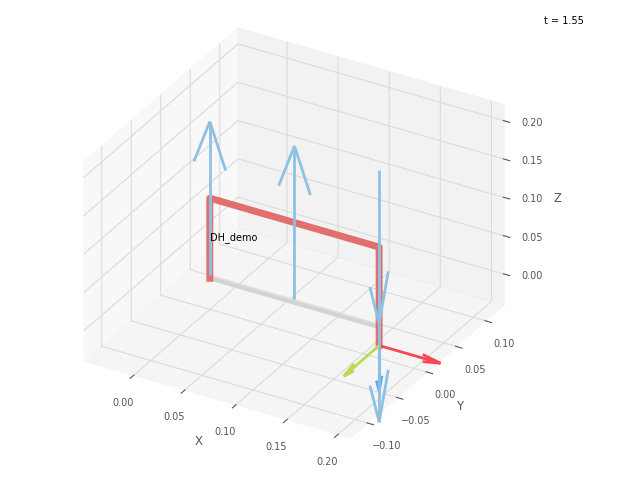
\includegraphics[width=.46\textwidth]{Robotics_Toolbox_for_Python_(Task0_1).png}}\hfill
\subfigure[Dofbot 五关节数学零位]{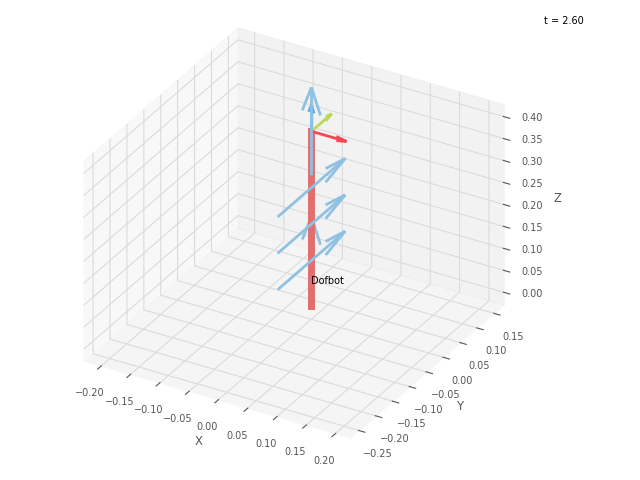
\includegraphics[width=.46\textwidth]{Robotics_Toolbox_for_Python_(Task0_2).png}}
\caption{任务 0 的 Robotics Toolbox 姿态图；后续计算使用右侧五关节模型}\label{fig:task0}
\end{figure}
\FloatBarrier

\section{任务 1：给定关节角的正运动学}
按 $\prod_{i=1}^{5}{}^{i-1}T_i$ 计算基座到 DH 末端坐标系的齐次变换。以下矩阵保留六位小数；数值极小的浮点项记为 0。矩阵右上角三维是末端位置，左上角 $3\times3$ 是旋转矩阵。

\subsection{Demo}
对 $q=[0,\pi/3,\pi/4,\pi/5,0]$，得到
\begin{equation}
T_{\mathrm{Demo}}=
\begin{bmatrix}
-0.777146&0&0.629320&0.232594\\
0&1&0&0\\
-0.629320&0&-0.777146&0.024681\\
0&0&0&1
\end{bmatrix}.
\end{equation}
\subsection{第 1 题}
对 $q=[\pi/2,\pi/5,\pi/5,\pi/5,\pi]$，得到
\begin{equation}
T_1=
\begin{bmatrix}
0&1&0&0\\
0.309017&0&0.951057&0.249628\\
0.951057&0&-0.309017&0.157445\\
0&0&0&1
\end{bmatrix}.
\end{equation}
\subsection{第 2 题}
对 $q=[\pi/3,\pi/4,-\pi/3,-\pi/4,\pi/2]$，得到
\begin{equation}
T_2=
\begin{bmatrix}
-0.866025&-0.250000&-0.433013&-0.037037\\
0.500000&-0.433013&-0.750000&-0.064150\\
0&-0.866025&0.500000&0.307321\\
0&0&0&1
\end{bmatrix}.
\end{equation}
\subsection{第 3 题}
对 $q=[-\pi/2,\pi/3,-2\pi/3,\pi/3,\pi/3]$，得到
\begin{equation}
T_3=
\begin{bmatrix}
0.866025&0.500000&0&0\\
-0.500000&0.866025&0&0\\
0&0&1&0.315770\\
0&0&0&1
\end{bmatrix}.
\end{equation}
\begin{figure}[!htbp]
\centering
\subfigure[Demo]{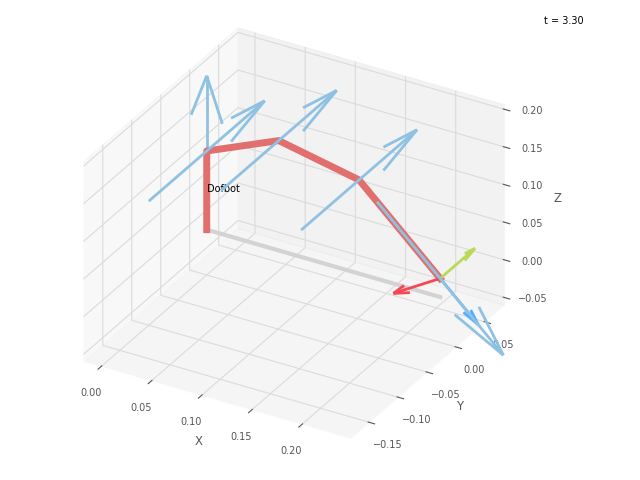
\includegraphics[width=.46\textwidth]{Robotics_Toolbox_for_Python_(Task1_1).png}}\hfill
\subfigure[第 1 题]{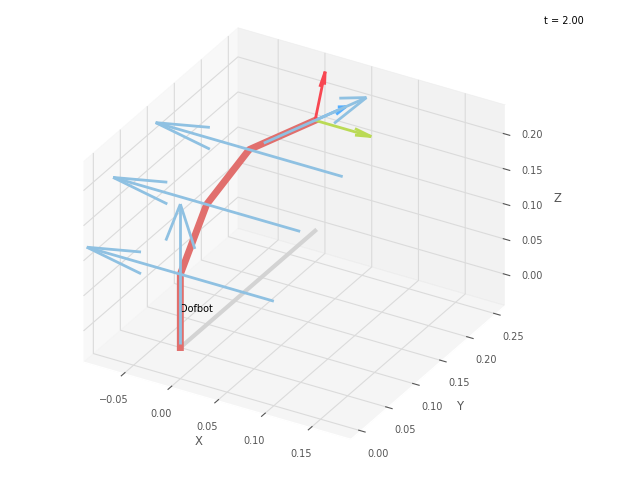
\includegraphics[width=.46\textwidth]{Robotics_Toolbox_for_Python_(Task1_2).png}}\\[0.6em]
\subfigure[第 2 题]{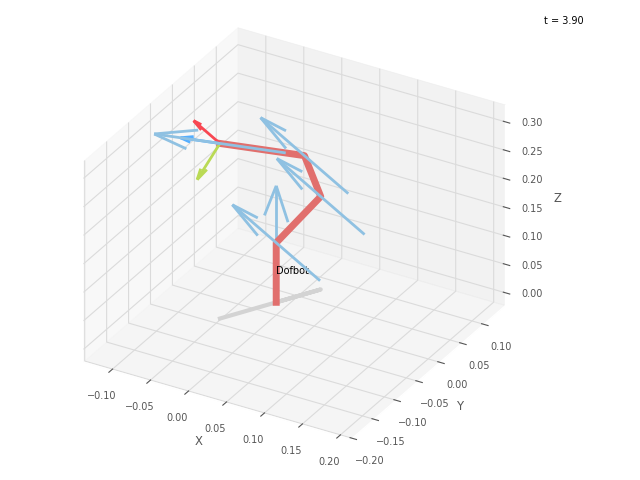
\includegraphics[width=.46\textwidth]{Robotics_Toolbox_for_Python_(Task1_3).png}}\hfill
\subfigure[第 3 题]{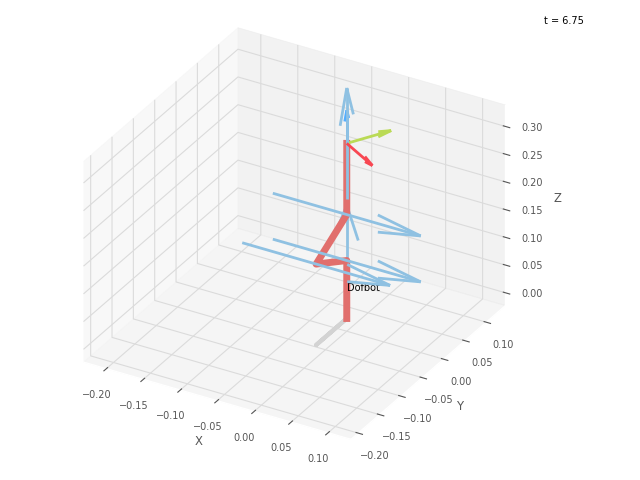
\includegraphics[width=.46\textwidth]{Robotics_Toolbox_for_Python_(Task1_4).png}}
\caption{任务 1 四组关节角对应的正运动学姿态}\label{fig:task1}
\end{figure}
四组矩阵的末端平移方向与图~\ref{fig:task1} 一致。第 2 题的 $q_4=-\pi/4<-0.16$\,rad，第 3 题的 $q_3=-2\pi/3<-1.05$\,rad，超出物理限位。这两组是题目指定的\textbf{数学正解}，不能直接当作实机指令。
\FloatBarrier

\section{任务 2：目标位姿的逆运动学}
三个正式目标使用 \texttt{ik\_LM}，共同初值为 $q_0=[0,\pi/2,\pi/2,\pi/2,\pi/2]$。返回关节解后用同一改进 DH 模型做 FK 复算。定义矩阵差及三种残差：
\begin{equation}
\Delta T=T_{\mathrm{FK}}-T_{\mathrm{target}},\quad
e_p=1000\|\Delta T_{1:3,4}\|_2,\quad
e_R=\|\Delta T_{1:3,1:3}\|_F,\quad
e_T=\|\Delta T\|_F .
\label{eq:ikresidual}
\end{equation}
$e_p$ 单位为 mm；$e_R$ 是矩阵差的 Frobenius 范数，\textbf{不是姿态角度误差}。计算时使用未四舍五入的关节解和目标数据。
\begin{table}[!htbp]
\centering\small
\caption{任务 2 三个正式目标的逆解汇总}\label{tab:iksummary}
\begin{tabular}{@{}cccccc@{}}
\toprule
目标 & 求解器成功 & $e_p$/mm & $e_R$ & $e_T$ & 物理限位\\ \midrule
1 & 是 & 0.997674 & $1.0532\times10^{-5}$ & 0.000997730 & 否，J4 越界\\
2 & 是 & 0.459553 & $7.1252\times10^{-6}$ & 0.000459608 & 是\\
3 & 是 & 0.714040 & $4.9052\times10^{-5}$ & 0.000715723 & 否，J2、J4 越界\\
\bottomrule
\end{tabular}
\end{table}

\subsection{目标 1：单位姿态}
目标位置为 $(0.1,0,0.1)$\,m，关节解（rad）为
\[
q\approx[0.000009,\,2.430481,\,0.132238,\,-2.562711,\,-0.000009].
\]
\begin{align}
T_{\mathrm{target},1}&=
\begin{bmatrix}1&0&0&0.1\\0&1&0&0\\0&0&1&0.1\\0&0&0&1\end{bmatrix},\\
T_{\mathrm{FK},1}&\approx
\begin{bmatrix}
1&0&0.000007&0.099401\\0&1&0&0.000001\\
-0.000007&0&1&0.100798\\0&0&0&1
\end{bmatrix},\\
\Delta T_1&\approx
\begin{bmatrix}
0&0&0.0000075&-0.0005991\\0&0&0&0.0000009\\
-0.0000075&0&0&0.0007978\\0&0&0&0
\end{bmatrix}.
\end{align}
主要误差来自 $x,z$ 平移。尽管数值求解成功，$q_4=-2.562711<-0.16$\,rad，故姿态图只说明 DH 数学解，不能证明实机可达。

\subsection{目标 2：绕 y 轴约 90°}
目标位置约为 $(0.241595205,0,0.217675205)$\,m，关节解（rad）为
\[
q\approx[0,\,1.057719,\,-0.544639,\,1.057711,\,0].
\]
\begin{align}
T_{\mathrm{target},2}&=
\begin{bmatrix}
0&0&1&0.241595205\\0&1&0&0\\-1&0&0&0.217675205\\0&0&0&1
\end{bmatrix},\\
T_{\mathrm{FK},2}&\approx
\begin{bmatrix}
0.000005&0&1&0.241270\\0&1&0&0\\-1&0&0.000005&0.217350\\0&0&0&1
\end{bmatrix},\\
\Delta T_2&\approx
\begin{bmatrix}
0.000005&0&0&-0.0003251\\0&0&0&0\\0&0&0.000005&-0.0003248\\0&0&0&0
\end{bmatrix}.
\end{align}
该组解在物理限位内，位置误差小于 0.5\,mm，是三组中兼具数值精度与关节可执行性的结果。

\subsection{目标 3：题面舍入的旋转矩阵}
关节解（rad）为
\[
q\approx[1.047197,\,-0.270573,\,1.064863,\,-1.841464,\,1.570790].
\]
\begin{align}
T_{\mathrm{target},3}&=
\begin{bmatrix}
-0.866&-0.250&-0.433&-0.03704\\
0.500&-0.433&-0.750&-0.06415\\
0&-0.866&0.500&0.30730\\0&0&0&1
\end{bmatrix},\\
T_{\mathrm{FK},3}&\approx
\begin{bmatrix}
-0.866024&-0.250016&-0.433007&-0.037128\\
0.500003&-0.433028&-0.749989&-0.064307\\
0.000005&-0.866013&0.500021&0.306609\\0&0&0&1
\end{bmatrix}.
\end{align}
完整矩阵差为
\begin{equation}
\Delta T_3\approx
\begin{bmatrix}
-0.0000237&-0.0000160&-0.0000068&-0.0000877\\
0.0000029&-0.0000278&0.0000106&-0.0001571\\
0.0000054&-0.0000132&0.0000211&-0.0006910\\
0&0&0&0
\end{bmatrix}.
\end{equation}
目标旋转矩阵的正交性误差 $\|R^\mathsf TR-I\|_F=7.7782\times10^{-5}$，源于题面小数舍入；前两组该误差为 0。本组虽然求解器返回成功，但 $q_2=-0.270573<0$、$q_4=-1.841464<-0.16$\,rad。

\begin{figure}[!htbp]
\centering
\subfigure[目标 1]{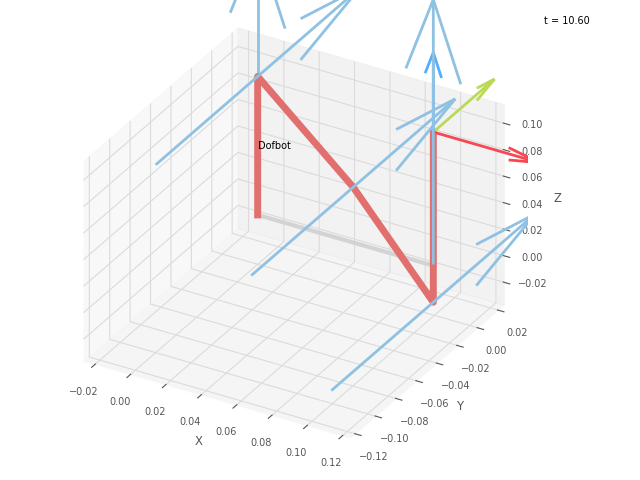
\includegraphics[width=.46\textwidth]{Robotics_Toolbox_for_Python_(Task2_1).png}}\hfill
\subfigure[目标 2]{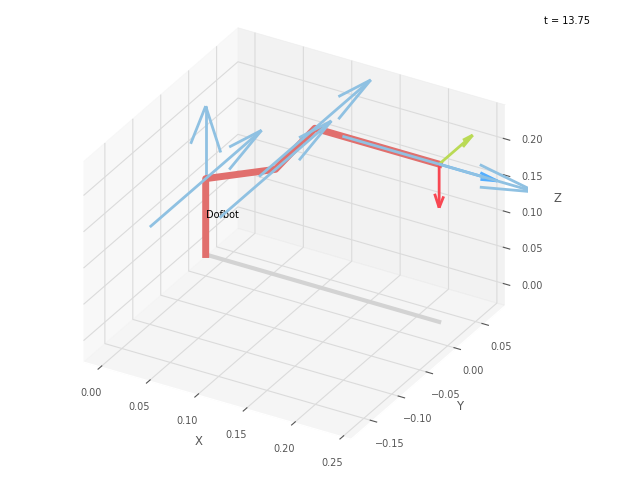
\includegraphics[width=.46\textwidth]{Robotics_Toolbox_for_Python_(Task2_2).png}}\\[0.6em]
\subfigure[目标 3]{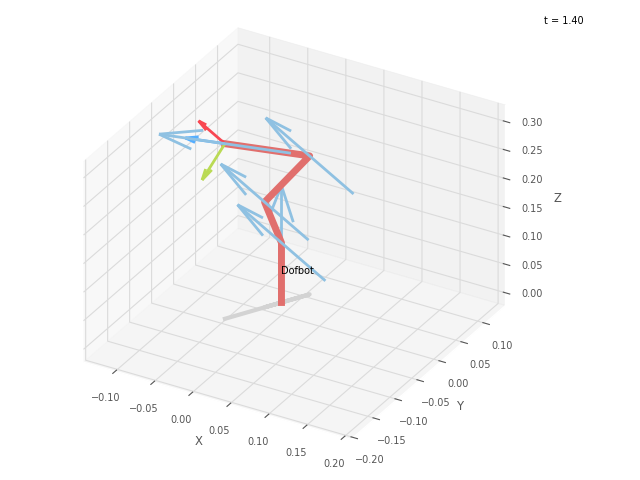
\includegraphics[width=.57\textwidth]{Robotics_Toolbox_for_Python_(Task2_3).png}}
\caption{任务 2 三组数值逆解对应的姿态图}\label{fig:task2}
\end{figure}
\texttt{ik\_LM} 的成功标志仅说明无物理限位约束的数学优化满足数值条件，不自动保证关节能执行。若用于实机，应在 IK 中加入关节限位或重选目标与初值，再做 FK 和碰撞复核。五自由度也不能独立满足任意六维位姿；若其他目标求解失败，应检查空间可达性、姿态相容性、关节限位、初值及旋转矩阵质量。本次三个正式目标没有求解器标记失败的案例。
\FloatBarrier

\section{任务 3：改进 DH 模型工作空间}
在表~\ref{tab:limits} 的范围内，对每个关节独立均匀采样，随机种子为 42。取 \texttt{num=30000} 组 $q$，逐组计算 DH 末端平移 $p(q)$，形成 $30000\times3$ 位置数组。输入角度单位为 rad，输出位置单位为 m；不做碰撞筛选。
\begin{table}[!htbp]
\centering\small
\caption{任务 3 与数据采集使用的物理关节范围}\label{tab:limits}
\begin{tabular}{@{}cccc@{}}
\toprule
关节 & 下限/rad & 上限/rad & 约略角度范围\\ \midrule
J1 & $-\pi$ & $\pi$ & $[-180^\circ,180^\circ]$\\
J2 & 0 & $\pi$ & $[0^\circ,180^\circ]$\\
J3 & $-1.05$ & $4.19$ & $[-60.16^\circ,240.07^\circ]$\\
J4 & $-0.16$ & $3.30$ & $[-9.17^\circ,189.08^\circ]$\\
J5 & $-\pi$ & $\pi$ & $[-180^\circ,180^\circ]$\\ \bottomrule
\end{tabular}
\end{table}
本次有限样本的极值为 $x\in[-0.290688,0.290572]$\,m、
$y\in[-0.292120,0.292320]$\,m、$z\in[-0.189042,0.398010]$\,m。图~\ref{fig:task3} 大体呈绕底座轴旋转的体积区域，与 J1 在 $[-\pi,\pi]$ 内转动相符。散点密度受关节空间均匀采样和运动学映射影响，不能视为笛卡尔空间均匀密度；样本极值也不是解析工作空间边界。
\begin{figure}[H]
\centering
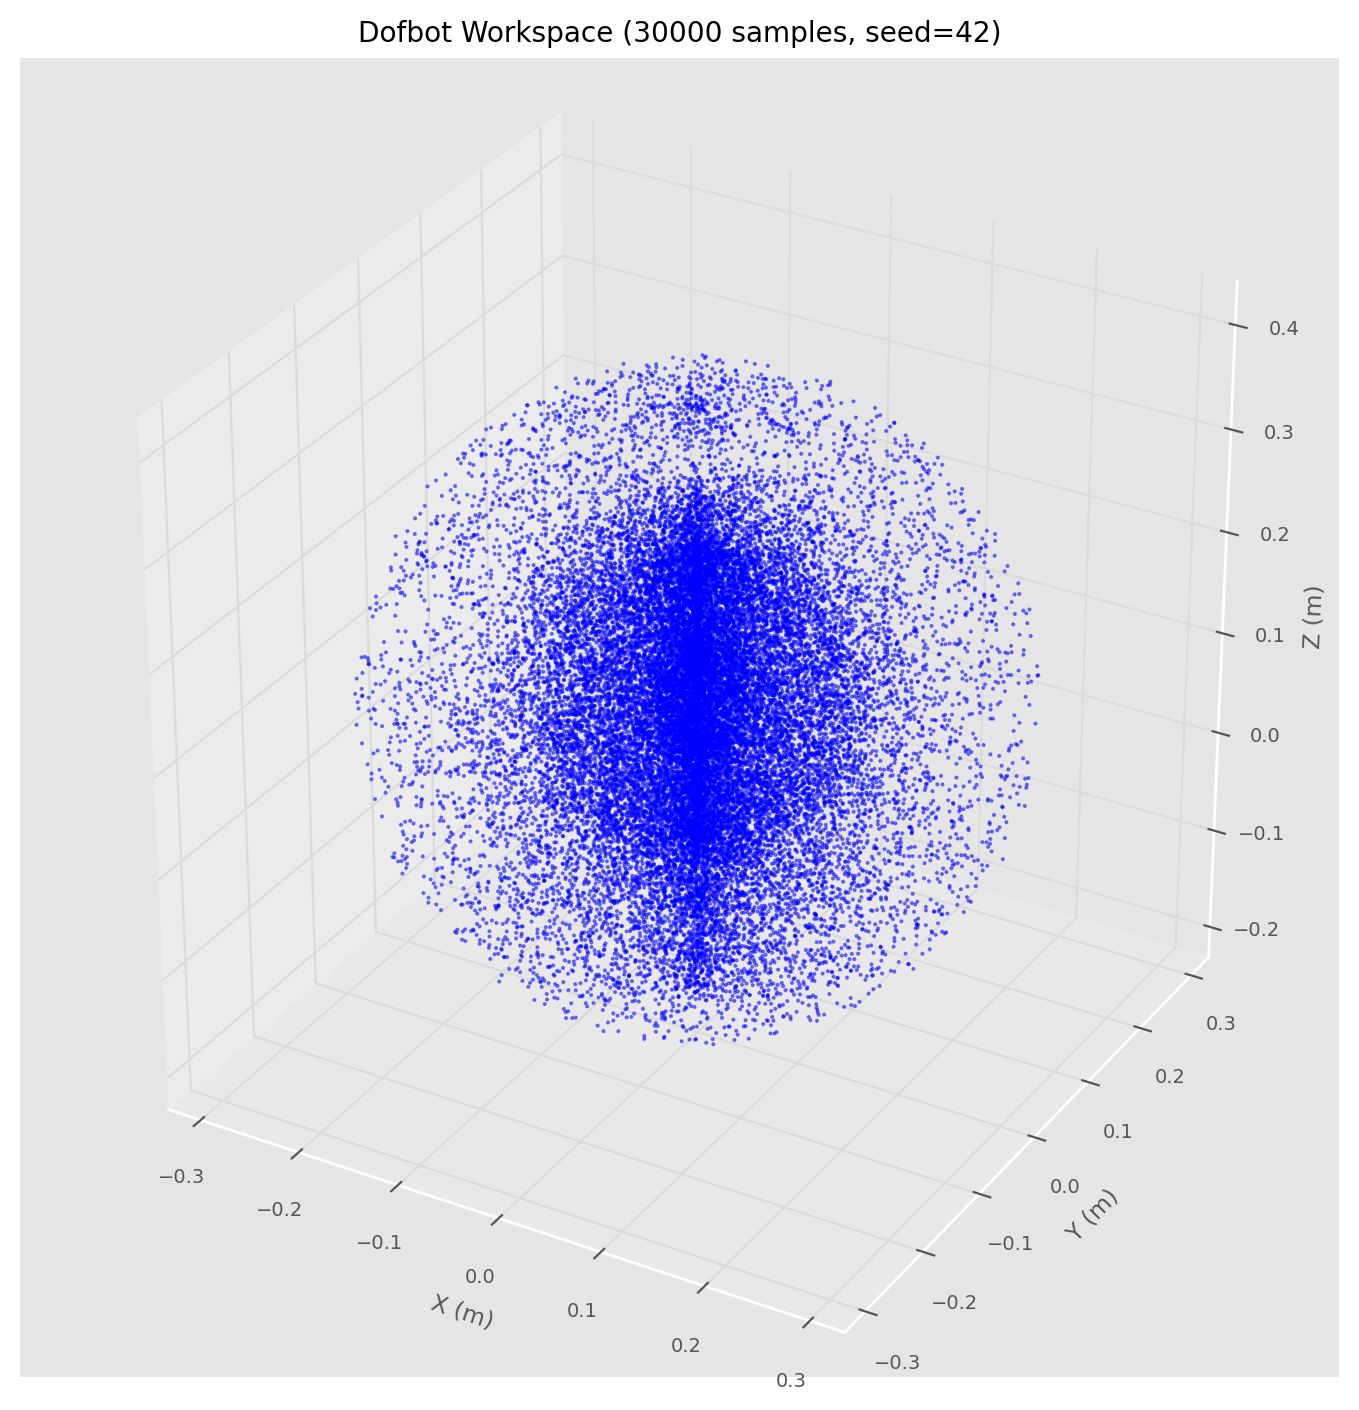
\includegraphics[width=.65\textwidth,height=.42\textheight,keepaspectratio]{task3_workspace.png}
\caption{30\,000 组改进 DH 末端位置形成的工作空间散点图}\label{fig:task3}
\end{figure}
\FloatBarrier

\section{任务 4：数据准备、归一化与空间观察}
使用项目已有的 \path{dataset/60000/dofbot_fk_60000_raw.csv}，共 60\,000 个样本。各关节在表~\ref{tab:limits} 的物理范围内独立均匀采样；PyBullet \texttt{DIRECT} 模式仅加载机械臂，直接设置关节状态，不加载桌子和物块、不做碰撞筛选。位姿采用 URDF 固定的 \texttt{tool\_center} TCP。原始 CSV 包含五关节角、TCP 的 XYZ、四元数、欧拉角和按列展开的旋转矩阵。
\begin{table}[!htbp]
\centering\small
\caption{60\,000 条数据的观测范围；为样本极值而非理论边界}\label{tab:data_range}
\begin{tabular}{@{}cccc@{}}
\toprule
量 & 最小值 & 最大值 & 单位\\ \midrule
J1 & -3.141535 & 3.141480 & rad\\
J2 & 0.000006 & 3.141557 & rad\\
J3 & -1.049931 & 4.189960 & rad\\
J4 & -0.159948 & 3.299978 & rad\\
J5 & -3.141420 & 3.141563 & rad\\
TCP $x$ & -0.267704 & 0.414261 & m\\
TCP $y$ & -0.339913 & 0.340904 & m\\
TCP $z$ & -0.151360 & 0.449590 & m\\ \bottomrule
\end{tabular}
\end{table}
周期角 J1、J5 用正余弦对表示；J2—J4 按物理关节范围线性映射到 $[-1,1]$，得到七维关节特征
\begin{equation}
u_q=[\sin q_1,\cos q_1,\tilde q_2,\tilde q_3,\tilde q_4,\sin q_5,\cos q_5].
\end{equation}
TCP 位姿采用十二维特征
\begin{equation}
u_T=[\tilde x,\tilde y,\tilde z,n_x,n_y,n_z,o_x,o_y,o_z,a_x,a_y,a_z],
\end{equation}
其中 $n,o,a$ 为旋转矩阵三列。XYZ 按数据统计的最小、最大值映射到 $[-1,1]$；旋转矩阵元素保持原尺度，原始四元数统一单位化。归一化数据和尺度参数分别保存为 \path{dataset/60000/dofbot_fk_60000_norm.csv} 与 \path{dataset/60000/dofbot_fk_60000_norm_stats.json}。
\begin{figure}[H]
\centering
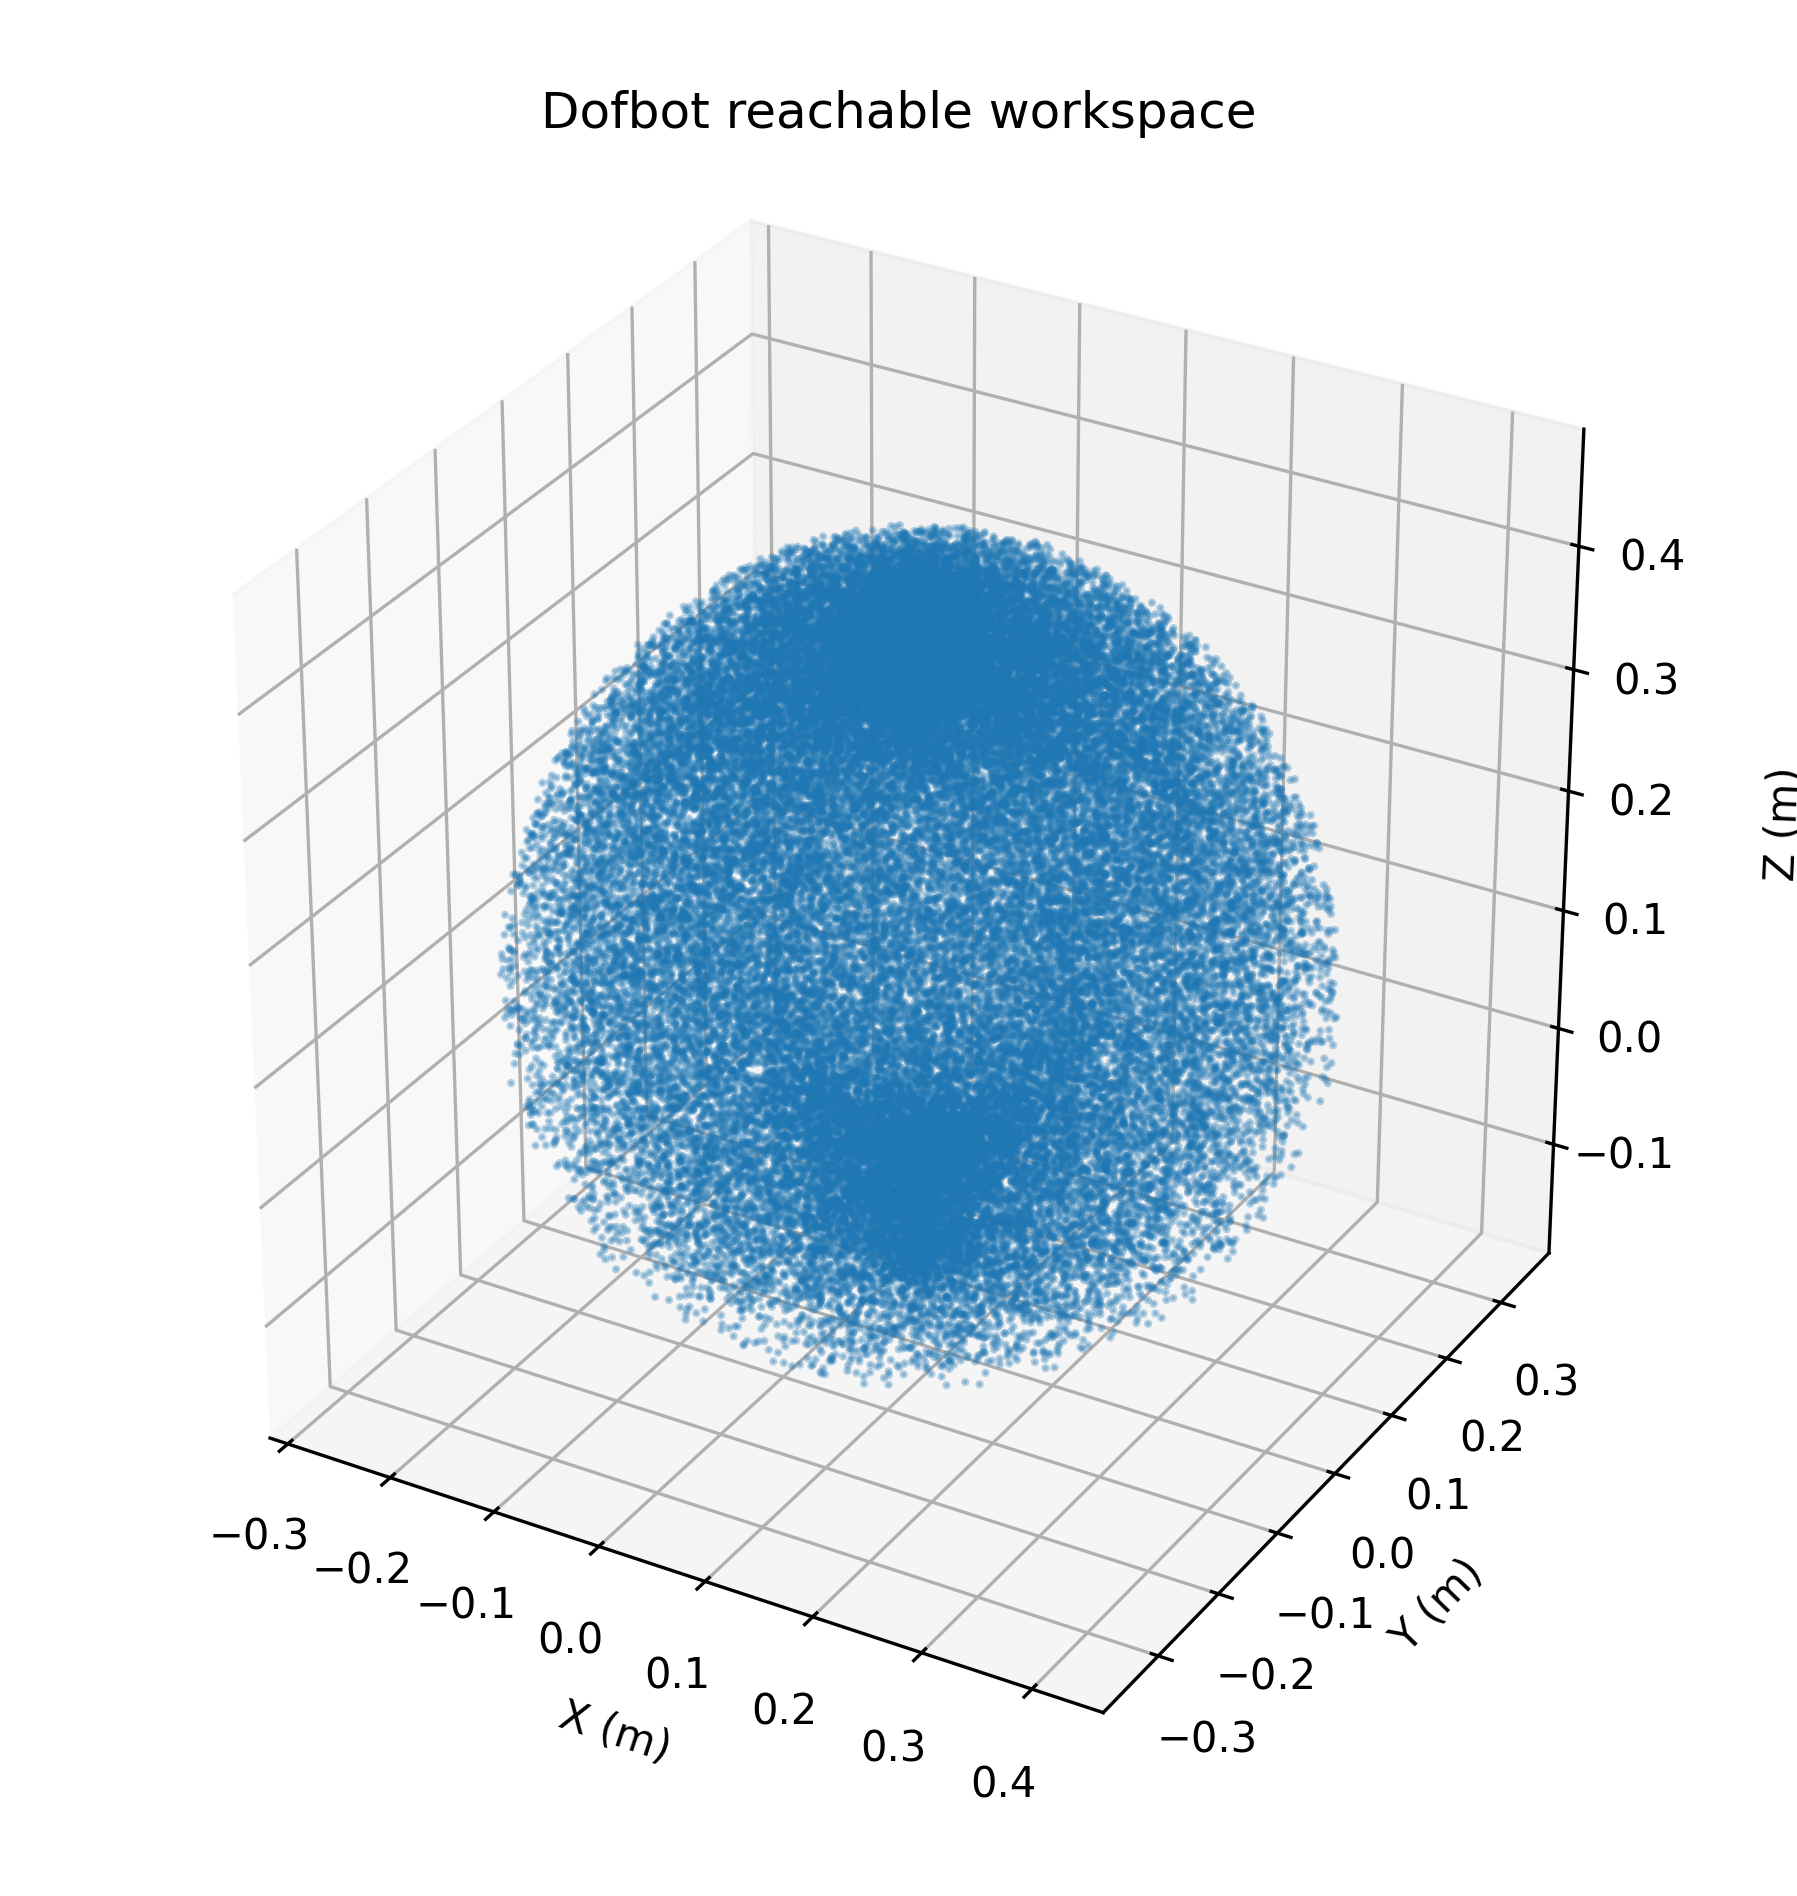
\includegraphics[width=.65\textwidth,height=.42\textheight,keepaspectratio]{task4_workspace_60000.png}
\caption{60\,000 条 PyBullet 数据中的 \texttt{tool\_center} TCP 位置}\label{fig:task4}
\end{figure}
图~\ref{fig:task4} 的坐标范围不能与图~\ref{fig:task3} 直接逐值比较：两图的末端坐标系及模型实现不同，也不能仅凭散点图判断 URDF 与 DH 的标定误差。
\FloatBarrier

\section{任务 5：FK/IK 网络训练}
\subsection{配置与训练方法}
\begin{table}[!htbp]
\centering\small
\caption{任务 5 的实际实验配置}\label{tab:train_config}
\begin{tabularx}{\textwidth}{@{}p{2.9cm}X@{}}
\toprule
项目 & 配置\\ \midrule
样本划分 & 60\,000 条；训练 48\,000、验证 12\,000（80\%/20\%）\\
网络结构 & \texttt{FlexibleMLP}；隐藏层宽度 $(128,128,64)$，使用线性层、LayerNorm、SiLU 与残差块\\
FK 映射 & 7 维关节特征 $\rightarrow$ 12 维 TCP 位姿\\
IK 映射 & 12 维 TCP 位姿 $\rightarrow 2\times7$ 维关节候选特征\\
轮数与批量 & 最多 200 轮；batch size 128\\
优化器与调度 & AdamW；初始学习率 $10^{-3}$，余弦退火至 $10^{-5}$；梯度范数上限 100\\
提前停止 & 验证损失连续 20 轮未改善则停止；每 20 轮保存检查点，同时保留最佳权重\\
随机种子与设备 & 训练种子 42；CPU\\
独立测试 & 1\,000 条新生成的可达目标；测试种子 2025\\ \bottomrule
\end{tabularx}
\end{table}
FK 直接学习关节特征到 TCP 位姿的映射。损失在反归一化后分别计算位置和旋转误差，以 10\,mm、5° 对应的物理尺度归一化，并加入权重 0.01 的旋转矩阵有效性约束。模型输出用于评估时投影到 $SO(3)$，使其正交且行列式为 $+1$。

IK 训练先冻结最佳 FK 网络，再使 IK 输出两个候选关节特征，分别经冻结 FK 重建位姿。对每个样本选择位姿损失较小的候选反向传播，即 \emph{best-of-2}。训练前 20\% 轮次加入初值为 0.01 且逐渐衰减到零的辅助关节监督；验证始终只计算位姿损失。推理时亦由学习 FK 的位姿损失选择候选，而非使用 PyBullet 真值挑选。

\subsection{训练结果与曲线}
\begin{table}[!htbp]
\centering\small
\caption{FK、IK 模型的实际训练结果}\label{tab:train_result}
\begin{tabular}{@{}ccccc@{}}
\toprule
模型 & 实际轮数 & 最佳轮次 & 最佳验证损失 & 提前停止\\ \midrule
FK & 200 & 199 & 0.00460333 & 否，达到最大轮数\\
IK & 62 & 42 & 0.13379793 & 是，20 轮无更低损失\\ \bottomrule
\end{tabular}
\end{table}
\begin{figure}[!htbp]
\centering
\subfigure[FK]{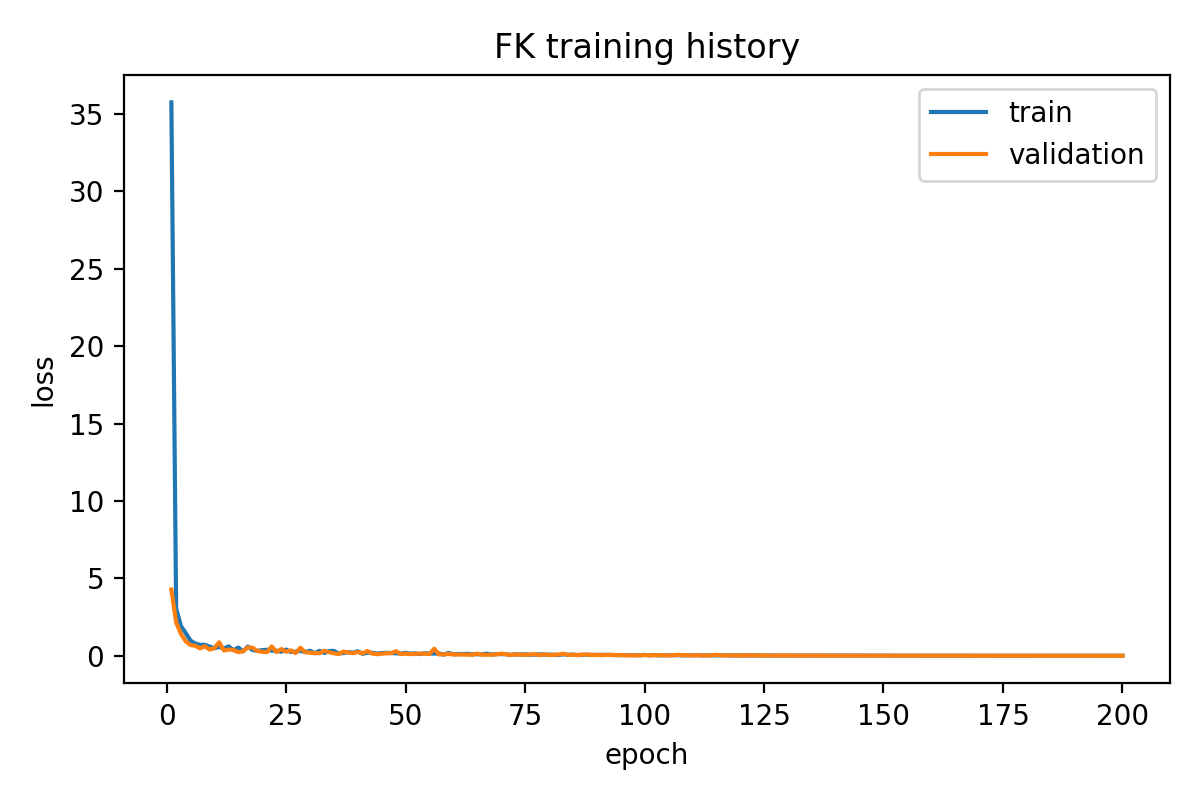
\includegraphics[width=.48\textwidth]{task5_fk_training_curve.png}}\hfill
\subfigure[IK]{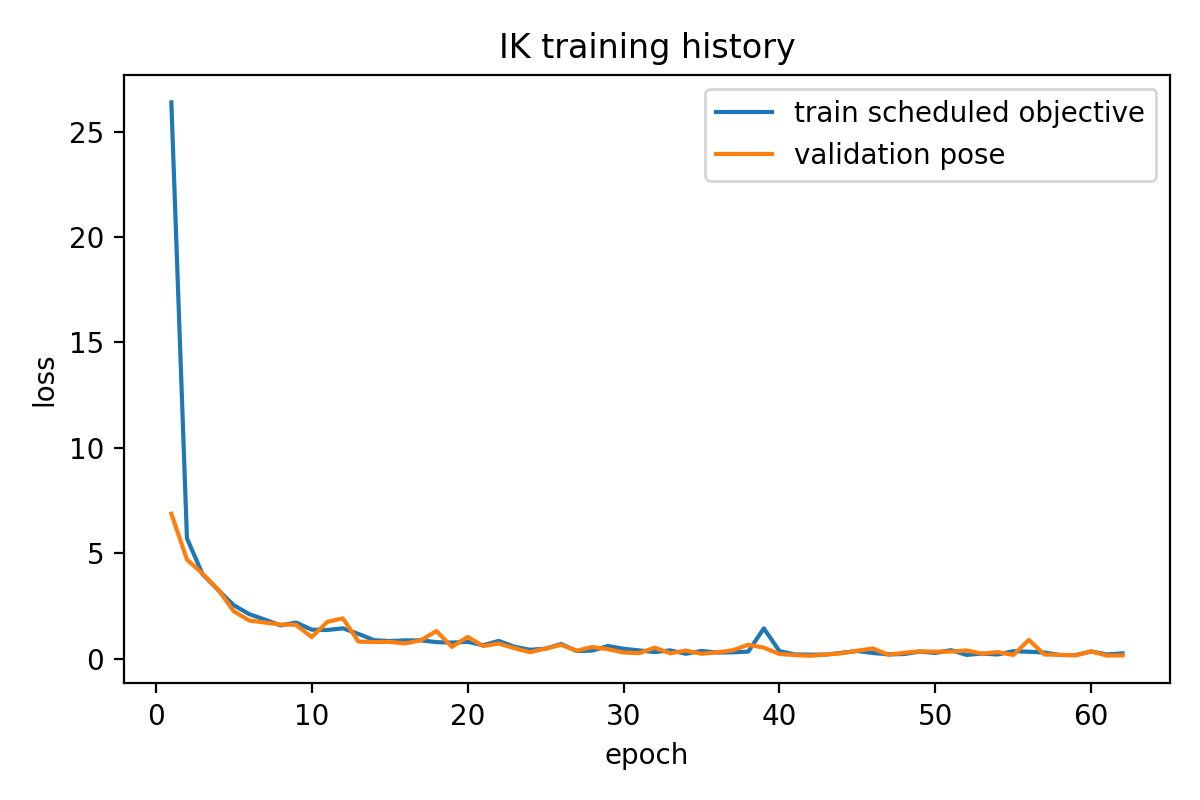
\includegraphics[width=.48\textwidth]{task5_ik_training_curve.png}}
\caption{训练与验证损失曲线}\label{fig:train_curve}
\end{figure}
FK 损失初期快速下降，后期持续缓慢收敛；第 199 轮取得最低验证损失 0.00460333，第 200 轮为 0.004676。曲线纵轴受首轮大损失影响，后段细节需结合数值。IK 在第 42 轮验证最优，随后波动并触发提前停止。IK 前 40 轮训练目标含逐渐衰减的辅助关节监督，验证只用位姿损失，因此早期两条曲线不宜逐点按相同损失项比较。

FK 较低的验证损失与后续测试精度一致。IK 损失更高且波动，与逆映射多解、候选选择和冻结 FK 的近似误差有关；仅从曲线不能断言过拟合。最优权重保存在相应时间戳目录的 \texttt{best\_model.pt} 中。
\FloatBarrier

\section{任务 6：评估函数、指标与误差分析}
\subsection{\texttt{evaluate\_pose()} 的定义}
函数输入两个形状为 $[N,12]$ 的数组。前三列是米制 XYZ，后九列为按列展开的旋转矩阵。比较前对预测和目标旋转矩阵做 SVD 投影到 $SO(3)$。对第 $i$ 个样本，定义
\begin{equation}
e_{p,i}=1000\|p_i^{\mathrm{pred}}-p_i^{\mathrm{target}}\|_2\quad(\mathrm{mm}),
\label{eq:positionerror}
\end{equation}
\begin{equation}
e_{R,i}=\frac{180}{\pi}\arccos\!\left[
\operatorname{clip}\!\left(
\frac{\operatorname{tr}\!\left((R_i^{\mathrm{pred}})^\mathsf T R_i^{\mathrm{target}}\right)-1}{2},
-1,1\right)\right]\quad (^\circ).
\label{eq:rotationerror}
\end{equation}
分别统计均值、中位数、总体标准差（\texttt{np.std}）、95\% 分位数和最大值。位置成功条件为 $e_p\leq10$\,mm，姿态成功条件为 $e_R\leq5^\circ$；\textbf{联合成功}要求两者同时成立。阈值与训练损失的物理尺度一致，便于比较训练目标与测试结果；它们不代表碰撞安全、夹取可靠性或所有应用的精度要求。

FK 比较网络预测与 PyBullet 真值。IK 将选出的关节角重新设置到 PyBullet，比较实际到达的 TCP 位姿与原目标，避免只用学习 FK 验证自身输出。
\subsection{独立测试结果}
\begin{table}[!htbp]
\centering\small
\caption{1\,000 条独立可达目标的误差统计}\label{tab:evaluation}
\begin{tabular}{@{}llrrrrrr@{}}
\toprule
模型 & 指标 & 均值 & 中位数 & 标准差 & P95 & 最大值 & 阈值内\\ \midrule
FK & 位置/mm & 0.495 & 0.448 & 0.265 & 0.967 & 1.888 & 100.0\%\\
FK & 姿态/$^\circ$ & 0.196 & 0.176 & 0.109 & 0.383 & 1.241 & 100.0\%\\
IK & 位置/mm & 3.389 & 3.028 & 2.029 & 6.674 & 26.389 & 99.0\%\\
IK & 姿态/$^\circ$ & 1.278 & 1.112 & 0.875 & 2.618 & 10.807 & 99.3\%\\
\bottomrule
\end{tabular}
\end{table}
FK 联合成功率为 \textbf{100.0\%（1000/1000）}，IK 为 \textbf{98.7\%（987/1000）}。IK 中有 10 条位置超出 10\,mm、7 条姿态超出 5°，其中 4 条同时超阈值，因此联合失败 13 条。
\begin{figure}[!htbp]
\centering
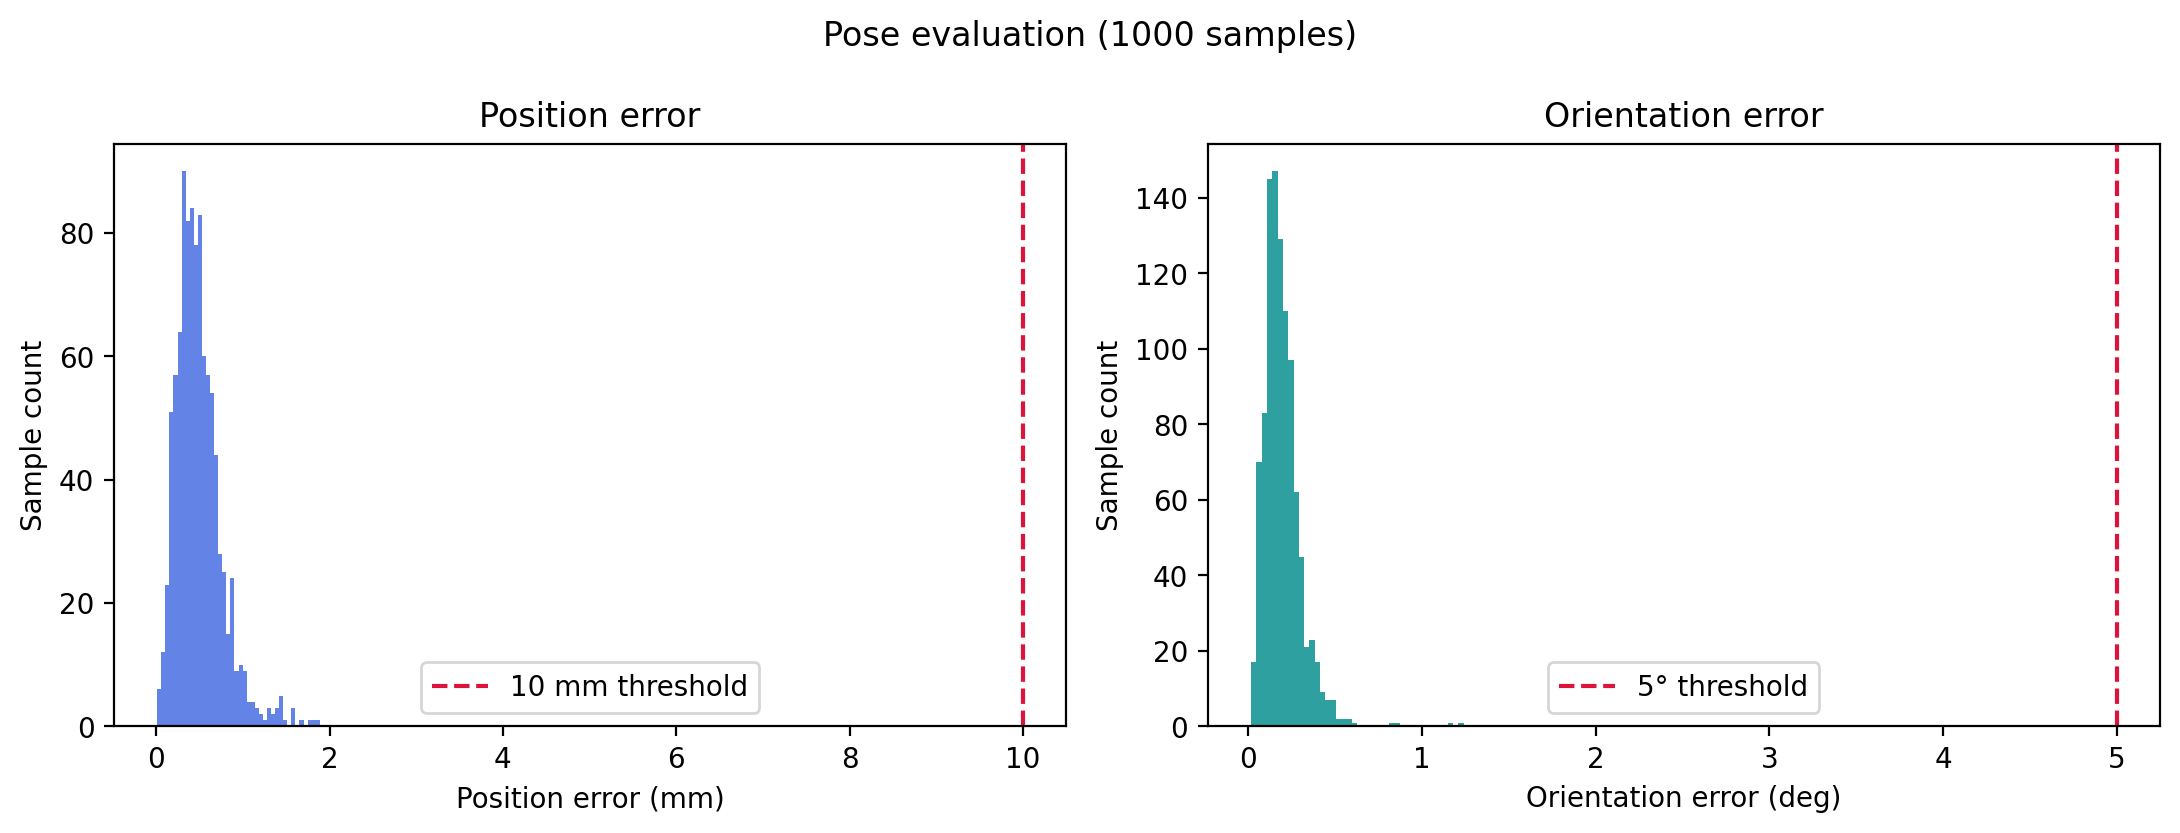
\includegraphics[width=.84\textwidth]{task6_fk_error.png}
\caption{FK 独立测试的位置与姿态误差分布；虚线对应 10\,mm 和 5°}\label{fig:fk_error}
\end{figure}
\begin{figure}[!htbp]
\centering
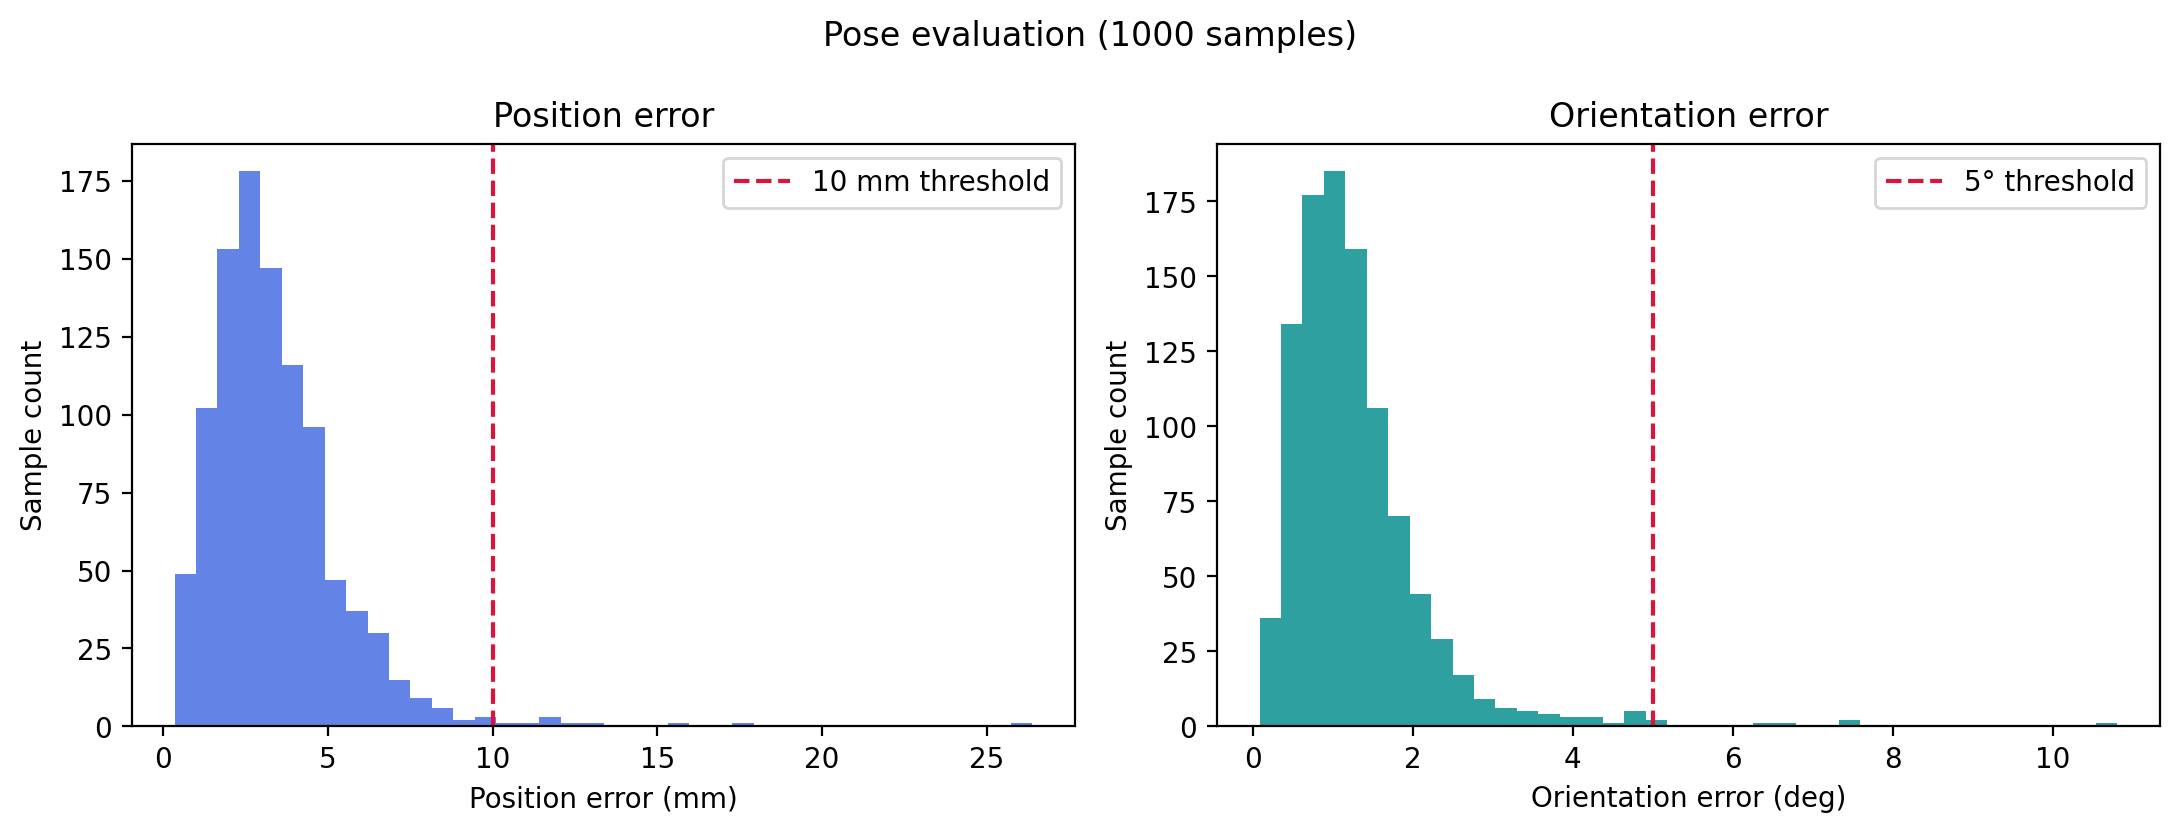
\includegraphics[width=.84\textwidth]{task6_ik_error.png}
\caption{IK 独立测试的位置与姿态误差分布；右尾有少量较差样本}\label{fig:ik_error}
\end{figure}
FK 的位置 P95 为 0.967\,mm、姿态 P95 为 0.383°，表明本次同分布测试集多数误差较小。IK 中位数为 3.028\,mm/1.112°，代表典型精度；最大值远高于 P95，平均值不足以描述困难样本。保存数据中，零基下标 786 的目标位置为 $(0.086447,0.016381,0.437041)$\,m，IK 位置误差 26.389\,mm、姿态误差约 4.328°，由位置项判失败；零基下标 633 的目标为 $(0.018185,0.015502,0.365492)$\,m，位置误差约 8.139\,mm、姿态误差约 10.807°，由姿态项判失败。两个阈值不能互相替代。

本次保存的 1\,000 条测试中，所选 IK 解均在代码规定的限位内；仍有失败样本，说明\textbf{关节合法不保证 TCP 位姿满足精度要求}。可能影响因素包括五自由度下的可达位姿约束、逆映射多解、有限候选数和学习 FK 的候选排序误差。若需确定具体原因，应逐样本检查雅可比条件数、局部训练样本密度及两个候选的真实 PyBullet 误差。统计只反映这次独立但同关节采样分布的可达目标，不代表跨 URDF 参数或实机的泛化性能。
\FloatBarrier

\section{任务 7：PyBullet 物块抓取与放置}
\subsection{场景、路点与控制}
正方体物块边长 0.03\,m，初始中心约为 $(0.2,0.1,0.015)$\,m，初始偏航角为 $\pi/6$；目标中心为 $(0.2,-0.1,0.015)$\,m。机械臂五关节从复位角开始，夹爪张开与闭合指令分别为 $+20^\circ$、$-20^\circ$。
程序读取物块和目标中心，在世界坐标系添加偏移形成表~\ref{tab:waypoints} 的 TCP 路点。
\begin{table}[!htbp]
\centering\small
\caption{成功运行记录的四个 TCP 目标路点}\label{tab:waypoints}
\begin{tabular}{@{}lll@{}}
\toprule
路点 & TCP 目标位置/m & 作用\\ \midrule
\texttt{pre\_grasp} & $(0.195,0.105,0.0649902)$ & 从上方接近及提起\\
\texttt{grasp} & $(0.195,0.105,0.0249902)$ & 下降夹取\\
\texttt{pre\_place} & $(0.200,-0.100,0.0650000)$ & 目标上方搬运及撤离\\
\texttt{place} & $(0.200,-0.100,0.0150000)$ & 下降释放\\ \bottomrule
\end{tabular}
\end{table}
每个路点调用 PyBullet 位置型 IK，检查五关节物理限位并用 PyBullet FK 复算；单路点容差为 15\,mm。程序记录期望的抓取与放置四元数，但\textbf{没有将完整姿态施加给 IK}：Dofbot 只有五个关节，无法独立指定任意六维 TCP 位姿，实际姿态由位置型 IK 解决定。J1、J5 沿跨 $\pm\pi$ 的较短角位移运动；每段关节角按
\begin{equation}
s(t)=10t^3-15t^4+6t^5,\qquad 0\leq t\leq1
\end{equation}
做五次平滑插值，历时 600 个仿真步。它使段首尾关节速度平滑，但\textbf{不保证 TCP 在笛卡尔空间走直线}。

动作顺序为接近、下降、闭合夹爪（400 步）、提升并检查物块离开桌面、搬运并再次确认物块被提起、下降、平滑打开夹爪（400 步）、抬起、回复位角、等待物块稳定。初期采用课程参考水平补偿时，夹爪只触及物块一侧；本次根据当前 URDF 的接触几何，将预抓取和抓取的水平偏移调为 $(-0.005,+0.005)$\,m，并以接触和提起结果核对；放置侧保持 $(0,0)$ 水平偏移。这个补偿是本仿真模型的标定结果，不能未经校准就移植到其他夹爪。

\subsection{实测误差与成功判据}
\begin{table}[!htbp]
\centering\small
\caption{抓放过程的 TCP 位置误差}\label{tab:pick_error}
\begin{tabular}{@{}lrr@{}}
\toprule
阶段 & IK/FK 复算/mm & 运动后实际误差/mm\\ \midrule
物块上方 & 8.38 & 8.38\\
下降抓取 & 1.11 & 1.11\\
提起物块 & 1.35 & 1.37\\
目标上方 & 2.00 & 1.99\\
下降放置 & 2.16 & 2.13\\
放置后抬起 & 1.68 & 1.68\\ \bottomrule
\end{tabular}
\end{table}
提起后物块中心为 $(0.19493,0.10226,0.04729)$\,m，高于桌面接触位置；搬运至目标上方后为 $(0.20193,-0.10282,0.04173)$\,m，显示物块随夹爪移动。最终稳定中心为 $(0.19723,-0.09742,0.01499)$\,m，与目标的三维距离为 \textbf{3.79\,mm}。这是\textbf{物块中心误差}，不同于表~\ref{tab:pick_error} 的 TCP 路点误差。

\texttt{task\_succeeded()} 要求物块水平中心距目标小于 10\,mm、竖直中心误差小于 10\,mm，并连续 100 帧保持线速度小于 0.02\,m/s、角速度小于 0.2\,rad/s；程序最多等待 1\,500 步。本次 GUI 运行输出“抓取放置成功”，最终位置与稳定判据一致。
\begin{figure}[!htbp]
\centering
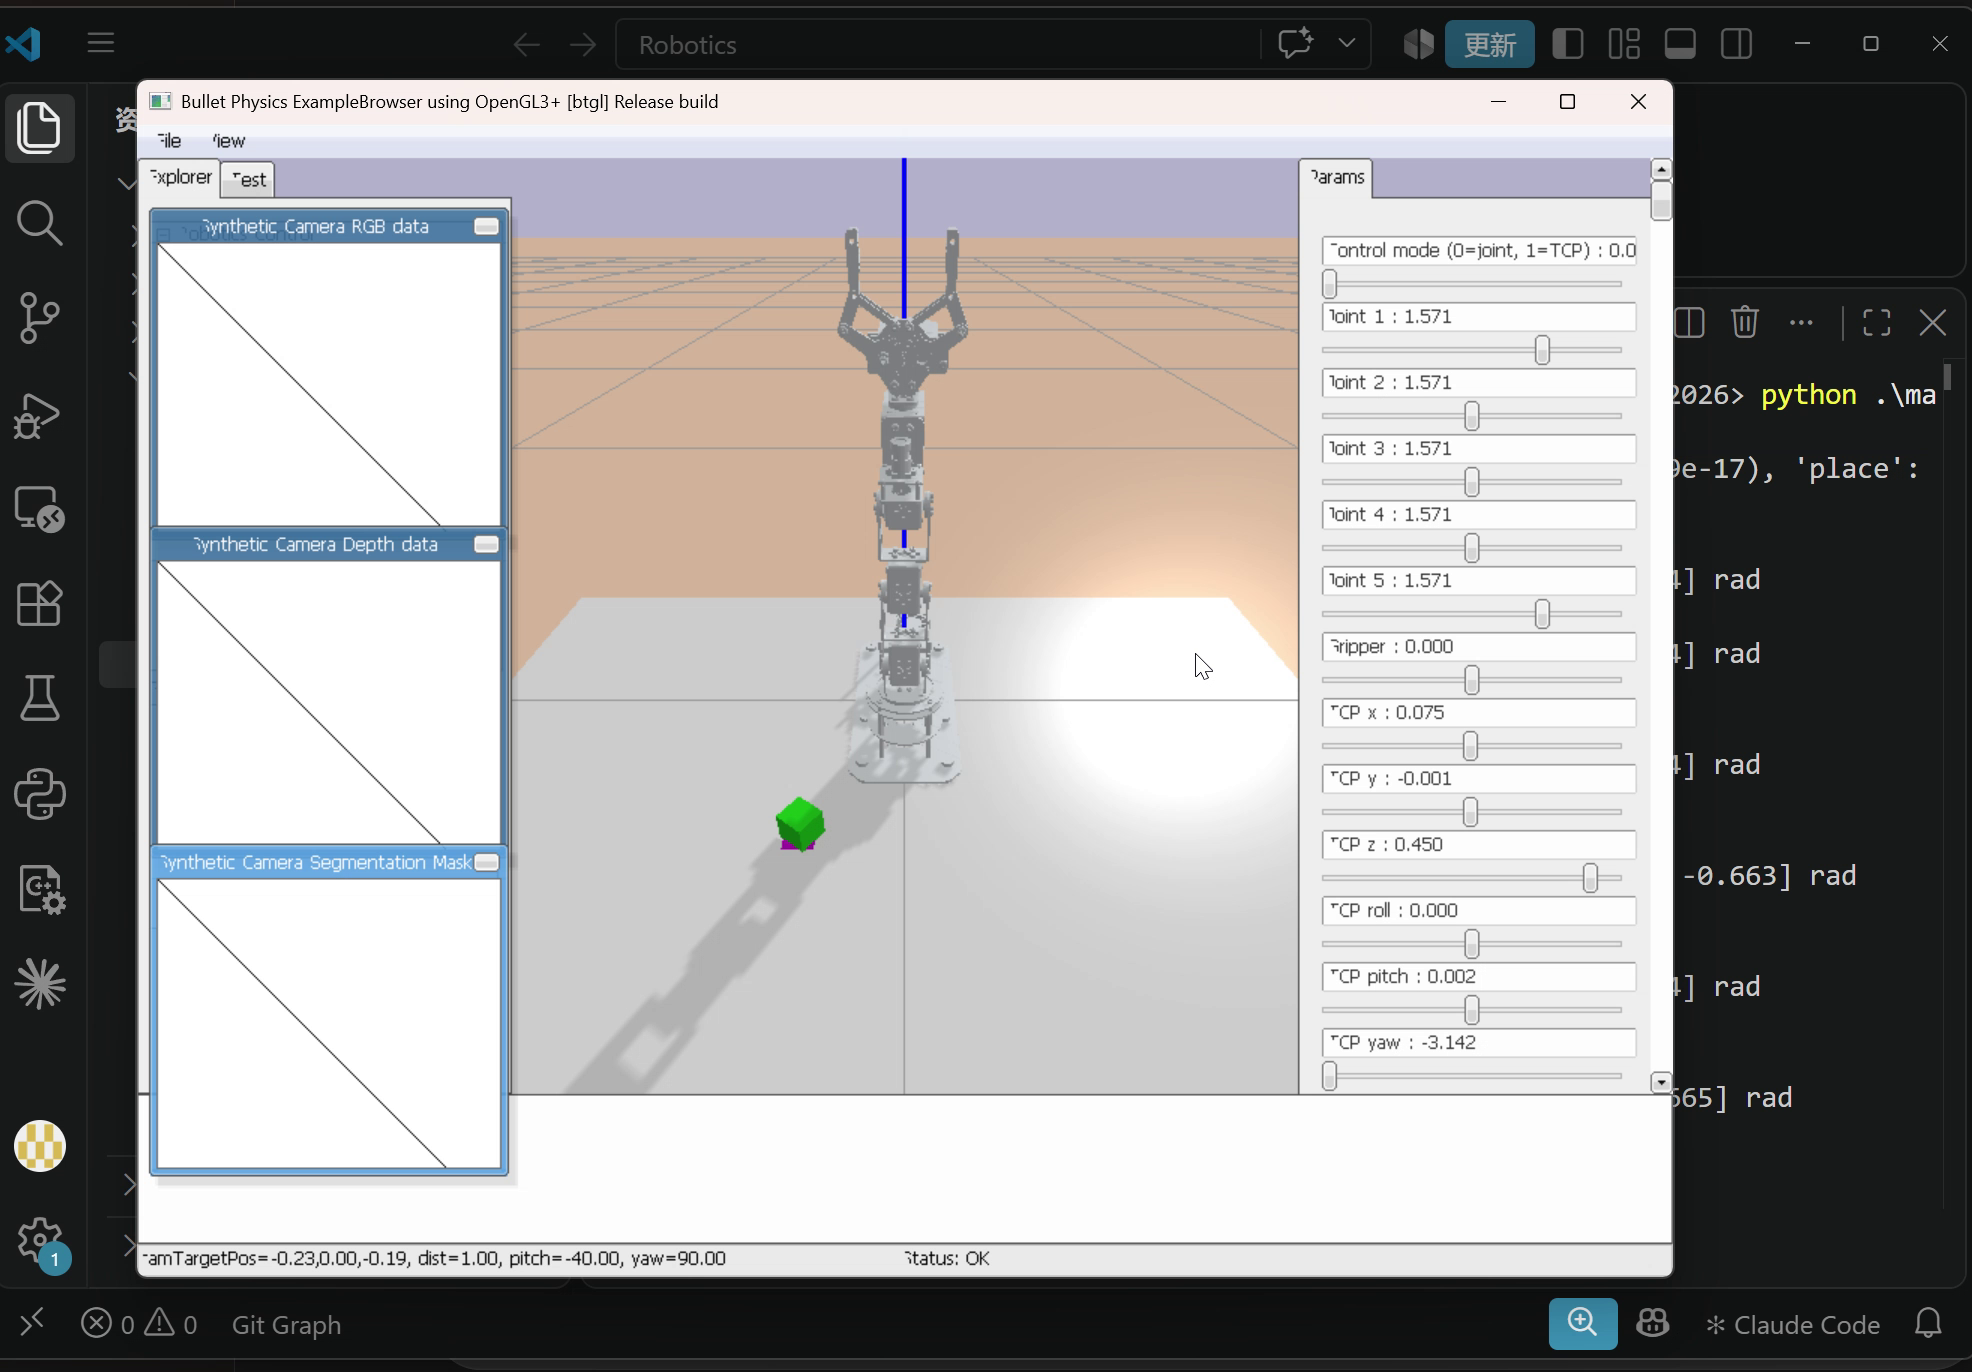
\includegraphics[width=.86\textwidth,height=.5\textheight,keepaspectratio]{task7_final_frame.png}
\caption{成功视频的最终场景：机械臂复位后，物块位于目标标记附近}\label{fig:task7}
\end{figure}
完整动作视频位于 \path{task7/task7.mp4}。带注释的实现文件为 \path{../main_student.py}；环境与成功判据见 \path{../dofbot.py}。

任务使用 PyBullet（动力学、IK、接触仿真）、NumPy（数组与轨迹插值）等第三方库。本次证据支持\textbf{该次仿真成功}；尚未对多随机种子或不同初始位置重复试验，不能据此估计长期抓取成功率。
\FloatBarrier

\section{综合讨论与结论}
改进 DH 模型使用所有给定几何参数，零位齐次变换与长度和相符；四组指定关节角的 FK 矩阵及姿态图形成对应证据。三个正式逆运动学目标在数学优化层面均有低残差解，但两组关节角越界，说明“求解器成功”“几何可达”“物理可执行”必须分别判断。

30\,000 点 DH 工作空间图满足课程最低采样量，并近似展示指定限位下的末端位置覆盖。60\,000 条 PyBullet \texttt{tool\_center} 数据用于训练 FK 与双候选 IK；FK 的独立测试误差低于 IK，后者在 1\,000 条测试中有 13 条联合超阈值。具体较差样本与误差分布显示，平均值之外仍需关注尾部误差。

抓放控制结合位置型 IK、关节平滑插值、接触标定和稳定判据，本次 GUI 仿真完成物块转移。若进一步面向真实机械臂，应统一 DH 末端与 URDF TCP 的标定，采用含关节限位及碰撞约束的 IK，检查全轨迹动力学可行性，并开展多次抓放试验统计成功率。

\paragraph{文件与复现入口}
任务 0—3 的源码为 \path{../dh_kine_student.py}，可用 \texttt{--task0-only} 至 \texttt{--task3-only} 分别运行。任务 4—6 的源码为 \path{../dofbot_learn_student.py}；结果保存在 \path{learn_model/}。任务 7 的源码与成功视频分别为 \path{../main_student.py}、\path{task7/task7.mp4}。本报告直接整理本次保存的实验结果；重新训练会产生新的随机结果和时间戳目录。
\end{document}
